\chapter{Synchronous Language Elements}\label{synchronous-language-elements}

This chapter defines synchronous
behavior suited for implementation of control systems.
The synchronous behavior relies on an additional kind of discrete-time
variables and equations, as well as an additional kind of when-clause.
The benefits of synchronous behavior is that it allows a model to define large
sampled data systems in a safe way, so that the
translator can provide good diagnostics in case of a modeling error.

The following small example shows the most important elements:
\begin{figure}[H]
  \begin{center}
    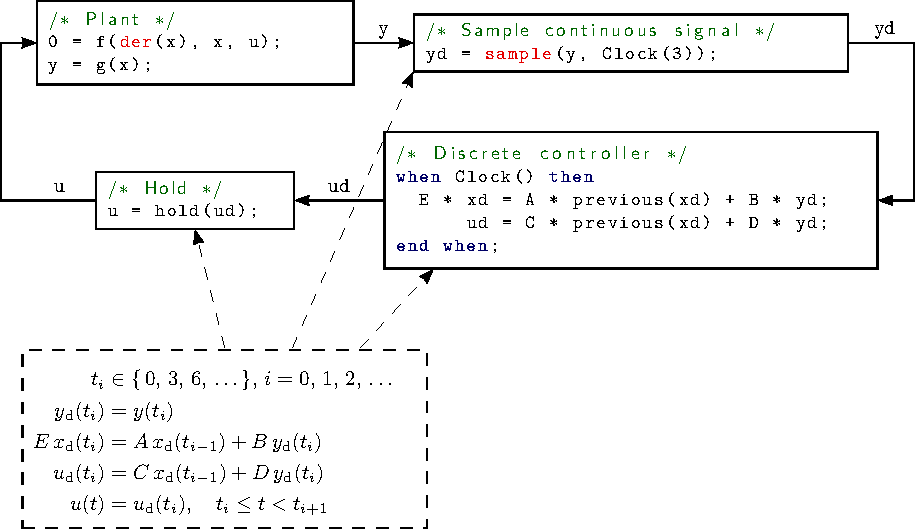
\includegraphics{plantmodel}
  \end{center}
  \caption{A continuous plant and a sampled data controller connected together with sample and (zero-order) hold elements.}
\end{figure}

\begin{itemize}
\item
  A periodic clock is defined with \lstinline!Clock(3)!. The argument
  of \lstinline!Clock! defines the sampling interval (for details see \cref{clock-constructors}).
\item
  Clocked variables (such as \lstinline!yd!, \lstinline!xd!, \lstinline!ud!) are associated uniquely
  with a clock and can only be directly accessed when the associated
  clock is active. Since all variables in a clocked equation must belong
  to the same clock, clocking errors can be detected at compile time. If
  variables from different clocks shall be used in an equation, explicit
  cast operators must be used, such as \lstinline!sample! to convert
  from continuous-time to clocked discrete-time or \lstinline!hold! to
  convert from clocked discrete-time to continuous-time.
\item
  A continuous-time variable is sampled at a clock tick with
  \lstinline!sample!. The operator returns the value of the
  continuous-time variable when the clock is active.
\item
  When no argument is defined for \lstinline!Clock!, the clock is
  deduced by clock inference.
\item
  For a \lstinline!when!-clause with an associated clock, all equations inside the \lstinline!when!-clause are clocked with the given clock.  All equations on an associated clock are treated together and in the same way regardless of whether they are inside a \lstinline!when!-clause or not.  This means that automatic sampling and hold of variables inside the \lstinline!when!-clause does not apply (explicit sampling and hold is required) and that general equations can be used in such when-clauses (this is not allowed for \lstinline!when!-clauses with \lstinline!Boolean! conditions, that require a variable reference on the left-hand side of an equation).
\item
  The \lstinline!when!-clause in the controller could also be removed
  and the controller could just be defined by the equations:
\begin{lstlisting}[language=modelica]
/* Discrete controller */
E * xd = A * previous(xd) + B * yd;
    ud = C * previous(xd) + D * yd;
\end{lstlisting}
\item
  \lstinline!previous(xd)! returns the value of \lstinline!xd! at
  the previous clock tick. At the first sample instant, the start value
  of \lstinline!xd! is returned.
\item
  A discrete-time signal (such as \lstinline!ud!) is converted to a continuous-time signal with \lstinline!hold!.
\item
  If a variable belongs to a particular clock, then all other equations where this variable is used, with the exception of as argument to certain special operators, belong also to this clock, as well as all variables that are used in these equations.
  This property is used for clock inference and allows defining an associated clock only at a few places (above only in the sampler, whereas in the discrete controller and the hold the sampling period is inferred).
\item
  The approach in this chapter is based on the clock calculus and inference system proposed by \textcite{ColacoPouzet2003ClocksFirstClass} and implemented in Lucid Synchrone version 2 and 3 \parencite{Pouzet2006LucidSynchrone30}.
  However, the Modelica approach also uses multi-rate periodic clocks based on rational arithmetic introduced by \textcite{ForgetEtAl2008MultiPeriodic}, as an extension of the Lucid Synchrone semantics.
  These approaches belong to the class of synchronous languages \parencite{BenvenisteEtAl2003SynchronousTwelveYearsLater}.
\end{itemize}
\section{Rationale for Clocked Semantics}\label{rationale-for-clocked-semantics}

\begin{nonnormative}
Periodically sampled control systems could also be defined with standard when-clauses, see \cref{when-equations}, and the \lstinline!sample! operator, see \cref{event-related-operators-with-function-syntax}.  For example:
\begin{lstlisting}[language=modelica]
when sample(0, 3) then
  xd = A * pre(xd) + B * y;
  u  = C * pre(xd) + D * y;
end when;
\end{lstlisting}

Equations in a when-clause with a \lstinline!Boolean! condition have the
property that (a) variables on the left hand side of the equal sign are
assigned a value when the when-condition becomes true and otherwise hold
their value, (b) variables not assigned in the when-clause are directly
accessed (= automatic \lstinline!sample! semantics), and (c) the variables
assigned in the when-clause can be directly accessed outside of the
when-clause (= automatic \lstinline!hold! semantics).

Using standard when-clauses works well for individual simple sampled blocks, but the synchronous approach using clocks and clocked equations provide the following benefits (especially for large sampled systems):
\begin{enumerate}
\item
  Possibility to detect inconsistent sampling rate, since clock partitioning (see \cref{clock-partitioning}),
  replaces the automatic sample and hold semantics. Examples:
  \begin{enumerate}
  \def\labelenumii{\alph{enumii}.}
  \item
    If when-clauses in different blocks should belong to the same
    controller part, but by accident different when-conditions are
    given, then this is accepted (no error is detected).
  \item
    If a sampled data library such as the
    Modelica\_LinearSystems2.Contoller library is used, at every block
    the sampling of the block has to be defined as integer multiple of a
    base sampling rate. If several blocks should belong to the same
    controller part, and different integer multiples are given, then the
    translator has to accept this (no error is detected).
  \end{enumerate}
  Note: Clocked systems can mix different sampling rates
  in well-defined ways when needed.
\item
  Fewer initial conditions are needed, as only a subset of clocked
  variables need initial conditions -- the clocked state variables (see \cref{clocked-state-variables}).
  For a standard when-clause all variables
  assigned in a when-clause must have an initial value
  because they might be used, before they are assigned a value the first
  time. As a result, all these variables are ``discrete-time states''
  although in reality only a subset of them need an initial
  value.
\item
  More general equations can be used, compared to standard when-clauses that require
  a restricted form of equations where the left hand side has to be a variable, in order
  to identify the variables that are assigned in the when-clause.
  This restriction can be circumvented for standard when-clauses, but is
  absent for clocked equations and make it more convenient to define
  nonlinear control algorithms.
\item
  Clocked equations allow clock inference,
  meaning that the sampling need only be given once for a sub-system.
  For a standard when-clause the condition (sampling) must be explicitly
  propagated to all blocks, which is tedious and error prone for large systems.
\item
  Possible to use general continuous-time models in synchronous models (e.g.\ some advanced controllers use an inverse model of a plant in the feedforward path of the controller, see \textcite{ThummelEtAl2005InverseModels}).
  This powerful feature of Modelica to use a nonlinear plant model in a controller would require to export the continuous-time model with an embedded integration method and then import it in an environment where the rest of the controller is defined.
  With clocked equations, clocked controllers with continuous-time models can be directly defined in Modelica.
\item
  Clocked equations are straightforward to optimize because they are
  evaluated exactly once at each an event instant.
  In contrast a standard when-clause with \lstinline!sample! conceptually
  requires several evaluations of the model (in some cases tools
  can optimize this to avoid unneeded evaluations).
  The problem for the standard when-clause is that after \lstinline!v!
  is changed, \lstinline!pre(v)! shall be updated and the model re-evaluated,
  since the equations could depend on \lstinline!pre(v)!.
  For clocked equations this iteration can be omitted
  since \lstinline!previous(v)! can only occur in the clocked equations
  that are only run the first event iterations.
\item
  Clocked subsystems using arithmetic blocks are straightforward to optimize.
  When a standard math-block (e.g.\ addition) is part of a clocked sub-system it is automatically
  clocked and only evaluated when the clocked equations trigger.
  For standard when-clauses one either needs a separate sampled math-block for each operation, or
  it will conceptually be evaluated all the time.
  However, tools may perform a similar optimization for standard when-clauses
  and it is only relevant in large sampled systems.
\end{enumerate}
\end{nonnormative}

\section{Definitions}\label{definitions}

In this section various terms are defined.

\subsection{Clocks and Clocked Variables}\label{clocks-and-clocked-variables}

% We can't use \subfloat just yet due to LaTeXML issue (fixed on master 2020-06-27):
%   https://github.com/brucemiller/LaTeXML/issues/1292 (marked as fixed as of commit 9f5c893b)
%\begin{figure}[tb]
%  \centering
%  \subfloat[A piecewise-constant variable.]{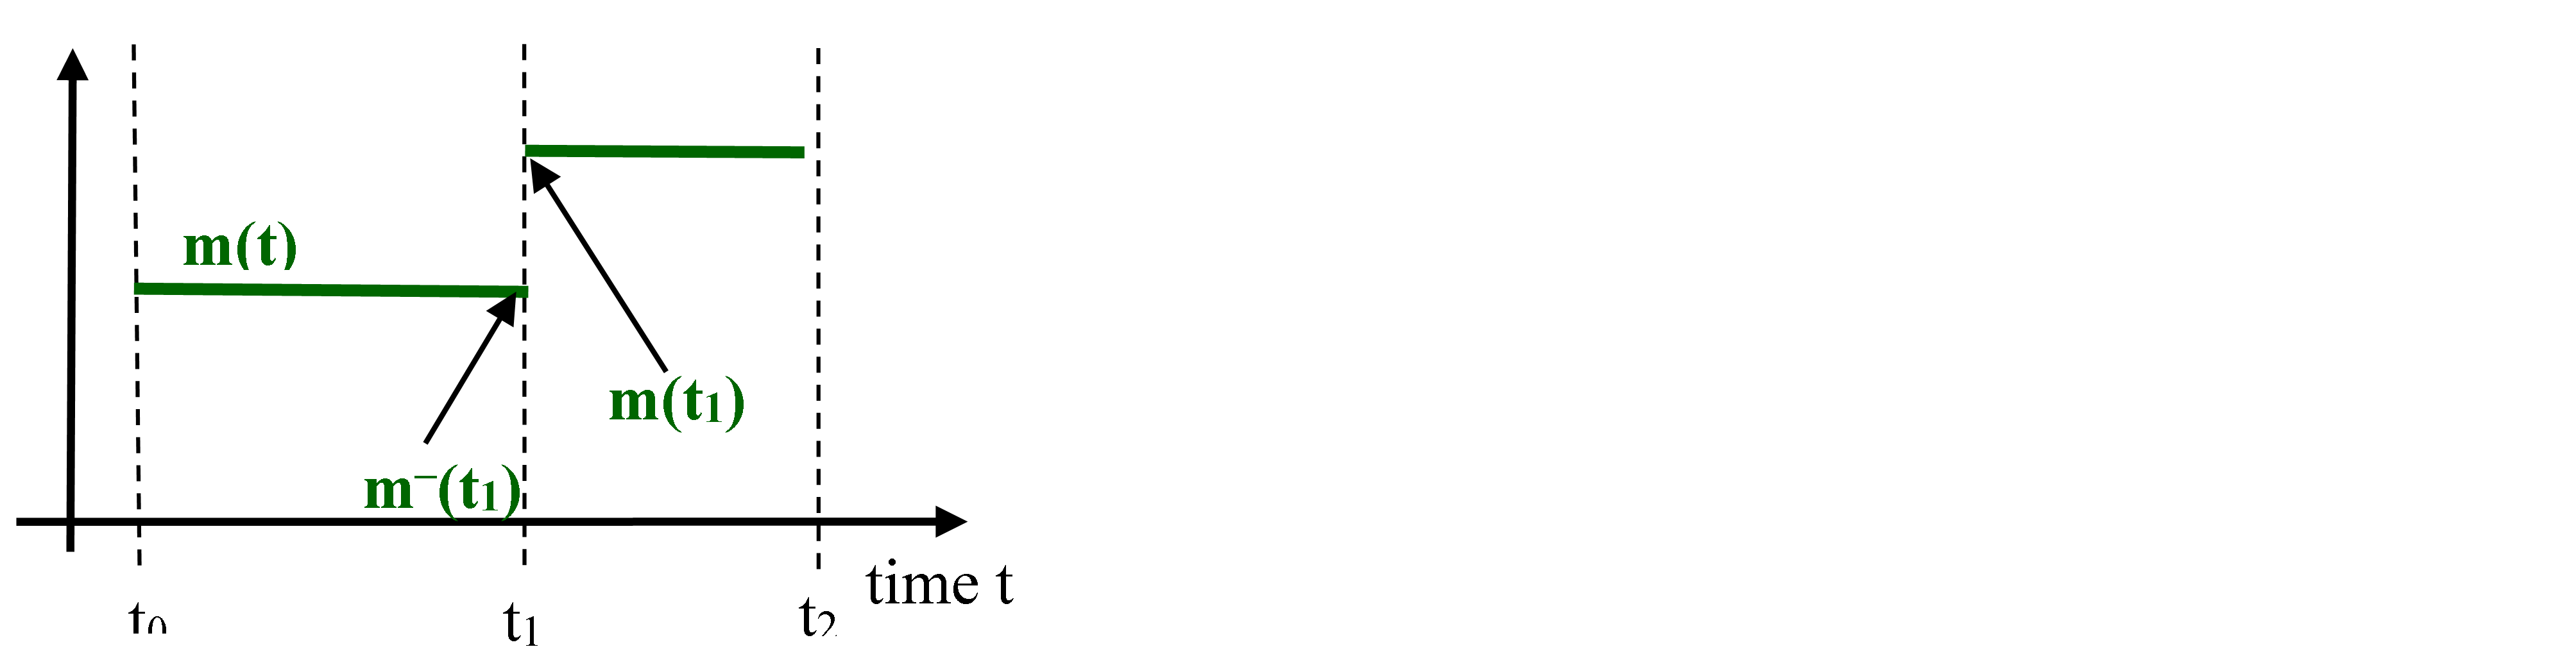
\includegraphics{piecewise}\label{fig:piecewise-constant-variable}}
%  \subfloat[A clock variable.]{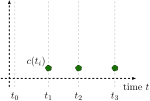
\includegraphics{clock}\label{fig:clock-variable}}
%  \subfloat[A clocked variable.]{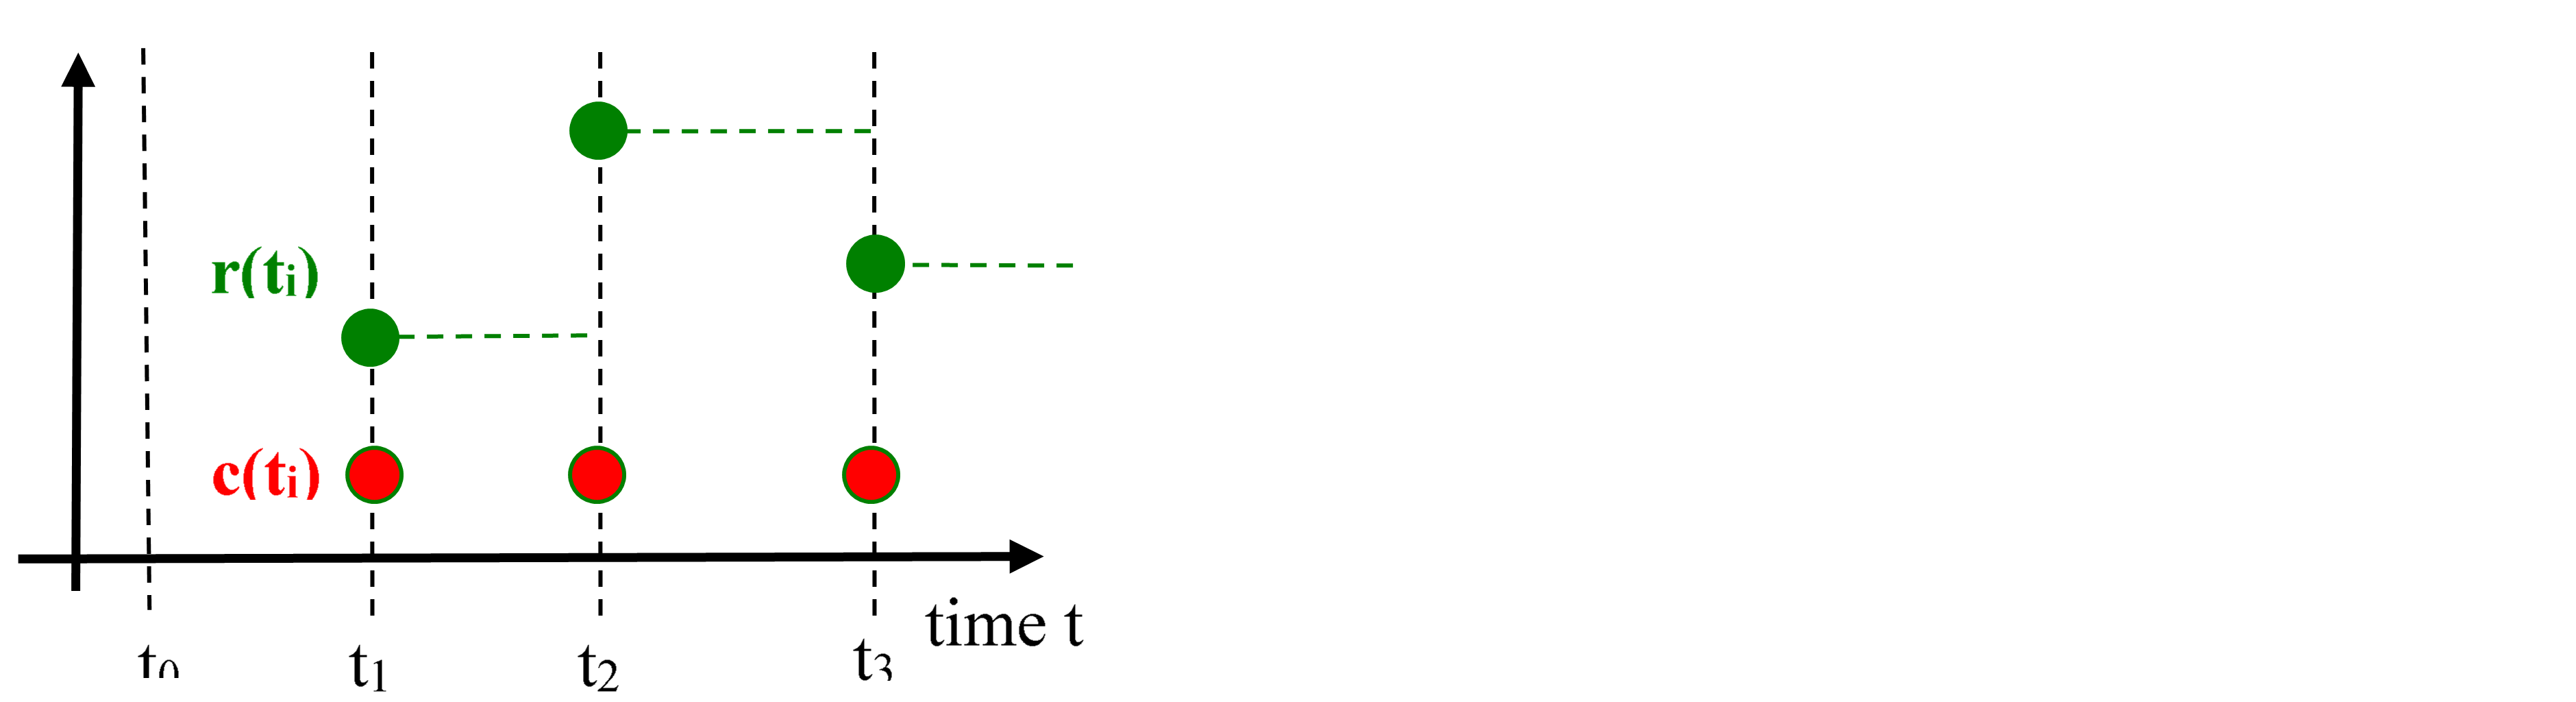
\includegraphics{clocked}\label{fig:clocked-variable}}
%  \caption{The different kinds of discrete-time variables.  The \lstinline!hold! extrapolation of the clocked variable is illustrated with dashed green lines.}
%\end{figure}

In \cref{discrete-time-expressions} the term \emph{discrete-time} Modelica expression and in \cref{continuous-time-expressions} the term \emph{continuous-time} Modelica expression is defined.
In this chapter, two additional kinds of discrete-time expressions/variables are defined that are associated to clocks and are therefore called \firstuse{clocked discrete-time}\index{clocked!discrete-time expression}\index{expression variability!clocked discrete-time} expressions.
The different kinds of discrete-time variables in Modelica are defined below.

\begin{definition}[Piecewise-constant variable]\index{piecewise-constant variable}
(See \cref{discrete-time-expressions}.)  Variables $m(t)$ of base type \lstinline!Real!, \lstinline!Integer!, \lstinline!Boolean!, enumeration, and \lstinline!String! that are
\emph{constant} inside each interval $t_{i} \leq t < t_{i+1}$ (i.e., piecewise constant continuous-time variables).  In other words, $m(t)$ changes
value only at events: $m(t) = m(t_{i})$, for $t_{i} \leq t < t_{i+1}$.  Such variables depend continuously on time and they are discrete-time variables.
See \cref{fig:piecewise-constant-variable}.
\end{definition}

\begin{figure}[H]
  \begin{center}
    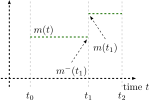
\includegraphics{piecewise-constant}
  \end{center}
  \caption{A piecewise-constant variable.}\label{fig:piecewise-constant-variable}
\end{figure}

\begin{definition}[Clock variable]\index{clock!variable}
Clock variables $c(t_{i})$ are of base type \lstinline!Clock!\indexinline{Clock}.
A clock is either defined by a constructor (such as \lstinline!Clock(3)!) that defines when the clock ticks (is active) at a particular time instant, or it is defined with clock operators relatively to other clocks, see \cref{base-clock-conversion-operators}.
See \cref{fig:clock-variable}.
\end{definition}

\begin{example}
Clock variables:
\begin{lstlisting}[language=modelica]
Clock c1 = Clock($\ldots$);
Clock c2 = c1;
Clock c3 = subSample(c2, 4);
\end{lstlisting}
\end{example}

\begin{figure}[H]
  \begin{center}
    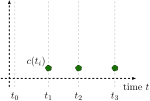
\includegraphics{clock}
  \end{center}
  \caption{A clock variable.  The value of a clock variable is not defined -- the plot marks only indicate \emph{when} the clock is active.}\label{fig:clock-variable}
\end{figure}

\begin{definition}[Clocked variable]\label{def:clocked-variable}\index{clocked!variable}
The elements of clocked variables $r(t_{i})$ are of base type \lstinline!Real!, \lstinline!Integer!, \lstinline!Boolean!, enumeration, \lstinline!String! that are associated uniquely with
a clock $c(t_{i})$. A clocked variable can only be directly accessed at the event instant where the associated clock is active.  A constant and a parameter can always be used at a place
where a clocked variable is required.
\begin{nonnormative}
Note that clock variables are not included in this list.
This implies that clock variables cannot be used where clocked variables are required.
\end{nonnormative}

At time instants where the associated clock is not active, the value of a clocked variable can be inquired by using an explicit cast operator, see below.  In such a case \lstinline!hold! semantics is
used, in other words the value of the clocked variable from the last event instant is used.  See \cref{fig:clocked-variable}.
\end{definition}

\begin{figure}[H]
  \begin{center}
    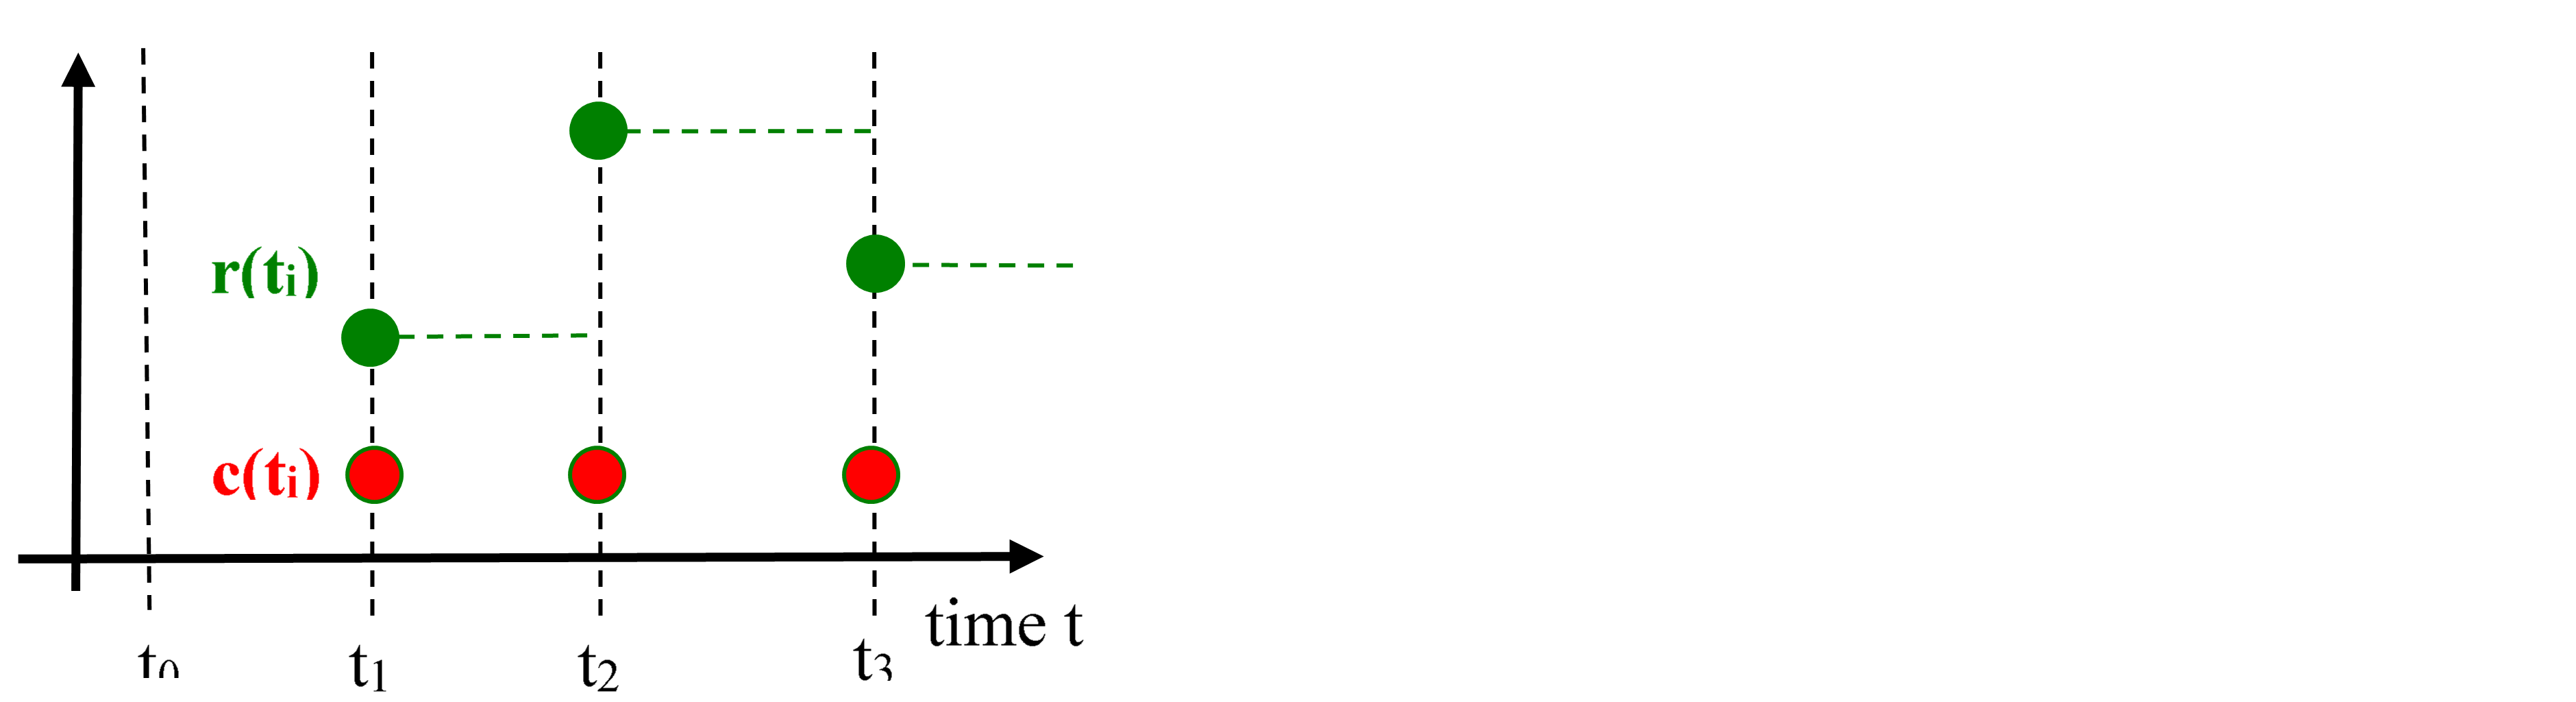
\includegraphics{clocked}
  \end{center}
  \caption{A clocked variable.  The \lstinline!hold! extrapolation of the value at the last event instant is illustrated with dashed green lines.}\label{fig:clocked-variable}
\end{figure}

\subsection{Base-Clock and Sub-Clock Partitions}\label{base-clock-and-sub-clock-partitions}

There are two kinds of \firstuse{clock partitions}\index{clock!partition}:

\begin{definition}[Base-clock partition]\index{base-clock partition}\index{clock!partition!base-clock}
A base-clock partition identifies a set of equations and a set of variables which must be executed together in one task.  Different base-clock partitions can be associated to separate tasks for
asynchronous execution.
\end{definition}

\begin{definition}[Sub-clock partition]\index{sub-clock partition}\index{clock!partition!sub-clock}
A sub-clock partition identifies a subset of equations and a subset of variables of a base-clock partition which are partially synchronized with other sub-clock partitions of the same base-clock
partition, i.e., synchronized when the ticks of the respective clocks are simultaneous.
\end{definition}

\subsection{Argument Restrictions (Component Expression)}\label{argument-restrictions-component-expression}

The built-in operators (with function syntax) defined in the following
sections have partially restrictions on their input arguments that are
not present for Modelica functions. To define the restrictions, the
following term is used.

\begin{definition}[Component expression]\label{def:component-expression}\index{component!expression (argument restriction)}
A component expression is a \lstinline[language=grammar]!component-reference! which is a valid expression, i.e., not referring to models or blocks with equations.
% "an element of records" below looks strange:
In detail, it is an instance of a (a) base type, (b) derived type, (c) record, (d) an array of such an instance (a-c), (e) one or more elements of such an array (d) defined by index expressions which are parameter expressions (see below), or (f) an element of records.
\begin{nonnormative}
The essential features are that one or several values are associated with the instance, that start values can be defined on these values, and that no equations are associated with the instance.
A component expression can be constant or can vary with time.
\end{nonnormative}
\end{definition}

In the following sections, when defining an operator with function calling syntax, there are some common restrictions being used for the input arguments (operands).
For example, an input argument to the operator may be required to be a component expression (\cref{def:component-expression}) or parameter expression (\cref{variability-of-expressions}).
To emphasize that there are no such restrictions, an input argument may be said to be just an \emph{expression}.

\begin{nonnormative}
The reason for restricting an input argument to be a component expression is that the start value of the input argument is returned before the first tick of the clock of the input argument and this
is not possible for a general expression.

The reason for restricting an input argument to be a parameter expression is that the value of the input argument needs to be evaluated during translation, in order that clock analysis can be performed during translation.
\end{nonnormative}

\begin{example}
The input argument to \lstinline!previous! is restricted to be a component expression.
\begin{lstlisting}[language=modelica]
Real u1;
Real u2[4];
Complex c;
Resistor R;
$\ldots$
y1 = previous(u1);    // fine
y2 = previous(u2);    // fine
y3 = previous(u2[2]); // fine
y4 = previous(c.im);  // fine
y5 = previous(2 * u); // error (general expression, not component expression)
y6 = previous(R);     // error (component, not component expression)
\end{lstlisting}
\end{example}

\begin{example}
The named argument \lstinline!factor! of \lstinline!subSample! is restricted to be a parameter expression.
\begin{lstlisting}[language=modelica]
Real u;
parameter Real p=3;
$\ldots$
y1 = subSample(u, factor = 3);         // fine (literal)
y2 = subSample(u, factor = 2 * p - 3); // fine (parameter expression)
y3 = subSample(u, factor = 3 * u);     // error (general expression)
\end{lstlisting}
\end{example}

None of the operators defined in this chapter vectorize, but some can operate directly on array variables (including clocked array variables, but not clock array variables).
They are not callable in functions.

\section{Clock Constructors}\label{clock-constructors}

The overloaded constructors listed below are available to generate clocks, and it is possible to call them with the specified named arguments, or with positional arguments (according to the order shown in the details after the table).
\begin{center}
\begin{tabular}{l|l l}
\hline
\tablehead{Expression} & \tablehead{Description} & \tablehead{Details}\\
\hline
\hline
\lstinline!Clock()! & Inferred clock & \Cref{modelica:clock-inferred}\\
\lstinline!Clock(intervalCounter, resolution)! & Rational interval clock & \Cref{modelica:clock-rational}\\
\lstinline!Clock(interval)! & Real interval clock & \Cref{modelica:clock-interval}\\
\lstinline!Clock(condition, startInterval)! & Event clock & \Cref{modelica:clock-event}\\
\lstinline!Clock(c, solverMethod)! & Solver clock & \Cref{modelica:clock-solver}\\
\hline
\end{tabular}
\end{center}

\begin{operatordefinition*}[Clock]\label{modelica:clock-inferred}\index{Clock@\robustinline{Clock}!inferred}
\begin{synopsis}\begin{lstlisting}
Clock()
\end{lstlisting}\end{synopsis}
\begin{semantics}
\firstuse{Inferred clock}\index{inferred clock}.
The operator returns a clock that is inferred.

\begin{example}
\begin{lstlisting}[language=modelica]
when Clock() then // equations are on the same clock
  x = A * previous(x) + B * u;
  Modelica.Utilities.Streams.print
    ("clock ticks at = " + String(sample(time)));
end when;
\end{lstlisting}
Note, in most cases, the operator is not needed and equations could be written without a when-clause (but not in the example above, since the \lstinline!print! statement is otherwise not associated to a clock).  This style is useful if a modeler would clearly like to mark the equations that must belong to one clock (although a tool could figure this out as well, if the when-clause is not present).
\end{example}
\end{semantics}
\end{operatordefinition*}

\begin{operatordefinition*}[Clock]\label{modelica:clock-rational}\index{Clock@\robustinline{Clock}!rational}
\begin{synopsis}\begin{lstlisting}
Clock(intervalCounter=$\mathit{intervalCounter}$, resolution=$\mathit{resolution}$)
\end{lstlisting}\end{synopsis}
\begin{semantics}
\firstuse{Rational interval clock}\index{rational interval clock}.
The first input argument, $\mathit{intervalCounter}$, is a clocked component expression (\cref{def:component-expression}) or a parameter expression of type \lstinline!Integer! with \lstinline!min = 0!.
The optional second argument $\mathit{resolution}$ (defaults to 1) is a parameter expression of type \lstinline!Integer! with \lstinline!min = 1! and \lstinline!unit = "Hz"!.
If $\mathit{intervalCounter}$ is a parameter expression with value zero, the period of the clock is derived by clock inference, see \cref{sub-clock-inferencing}.

If $\mathit{intervalCounter}$ is a parameter expression greater than zero, the clock defines a periodic clock.
If $\mathit{intervalCounter}$ is a clocked component expression it must be greater than zero.
The result is of base type \lstinline!Clock! that ticks when \lstinline!time! becomes $t_{\mathrm{start}}$, $t_{\mathrm{start}} + \mathit{interval}_{1}$, $t_{\mathrm{start}} + \mathit{interval}_{1} + \mathit{interval}_{2}$, \@\ldots{}
The clock starts at the start of the simulation $t_{\mathrm{start}}$ or when the controller is switched on.
At the start of the simulation, \lstinline!previous($\mathit{intervalCounter}$)! = \lstinline!$\mathit{intervalCounter}$.start! and the clocks ticks the first time.
At the first clock tick $\mathit{intervalCounter}$ must be computed and the second clock tick is then triggered at $\mathit{interval}_{1} = \mathit{intervalCounter}/\mathit{resolution}$.
At the second clock tick at time $t_{\mathrm{start}} + \mathit{interval}_{1}$, a new value for $\mathit{intervalCounter}$ must be computed and the next clock tick is scheduled at $\mathit{interval}_{2} = \mathit{intervalCounter}/\mathit{resolution}$, and so on.


\begin{nonnormative}
The given interval and time shift % What given "interval" and "time shift"?
can be modified by using the \lstinline!subSample!, \lstinline!superSample!, \lstinline!shiftSample! and \lstinline!backSample! operators on the returned clock, see \cref{sub-clock-conversion-operators}.
\end{nonnormative}

\begin{example}
\begin{lstlisting}[language=modelica]
  // first clock tick: previous(nextInterval) = 2
  Integer nextInterval(start = 2);
  Real y1(start = 0);
  Real y2(start = 0);
equation
  when Clock(2, 1000) then
    // periodic clock that ticks at 0, 0.002, 0.004, $\ldots$
    y1 = previous(y1) + 1;
  end when;

  when Clock(nextInterval, 1000) then
    // interval clock that ticks at 0, 0.003, 0.007, 0.012, $\ldots$
    nextInterval = previous(nextInterval) + 1;
    y2 = previous(y2) + 1;
  end when;
\end{lstlisting}
\end{example}

Note that operator \lstinline!interval(c)! of \lstinline!Clock c = Clock(nextInterval, $\mathit{resolution}$)! returns:\newline
\lstinline!previous($\mathit{intervalCounter}$) / $\mathit{resolution}$! (in seconds)
\end{semantics}
\end{operatordefinition*}

\begin{operatordefinition*}[Clock]\label{modelica:clock-interval}\index{Clock@\robustinline{Clock}!interval}
\begin{synopsis}\begin{lstlisting}
Clock(interval=$\mathit{interval}$)
\end{lstlisting}\end{synopsis}
\begin{semantics}
\firstuse{Real interval clock}\index{real interval clock}.
The input argument, $\mathit{interval}$, is a clocked component expression (\cref{def:component-expression}) or a parameter expression.
The $\mathit{interval}$ must be strictly positive ($\mathit{interval} > 0$) of type \lstinline!Real! with \lstinline!unit = "s"!.
The result is of base type \lstinline!Clock! that ticks when \lstinline!time! becomes $t_{\mathrm{start}}$, $t_{\mathrm{start}} + \mathit{interval}_{1}$, $t_{\mathit{start}} + \mathit{interval}_{1} + \mathit{interval}_{2}$, \@\ldots{}
The clock starts at the start of the simulation $t_{\mathrm{start}}$ or when the controller is switched on.
Here the next clock tick is scheduled at $\mathit{interval}_{1}$ = \lstinline!previous($\mathit{interval}$)! = \lstinline!$\mathit{interval}$.start!.
At the second clock tick at time $t_{\mathrm{start}} + \mathit{interval}_{1}$, the next clock tick is scheduled at $\mathit{interval}_{2}$ = \lstinline!previous($\mathit{interval}$)!, and so on.
If $\mathit{interval}$ is a parameter expression, the clock defines a periodic clock.

\begin{nonnormative}
Note, the clock is defined with \lstinline!previous($\mathit{interval}$)!.  Therefore, for sorting the input argument is treated as known.  The given interval and time shift can be modified by using the \lstinline!subSample!, \lstinline!superSample!, \lstinline!shiftSample! and \lstinline!backSample! operators on the returned clock, see \cref{sub-clock-conversion-operators}.  There are restrictions where this operator can be used, see \lstinline!Clock! expressions below.
\end{nonnormative}
\end{semantics}
\end{operatordefinition*}

\begin{operatordefinition*}[Clock]\label{modelica:clock-event}\index{Clock@\robustinline{Clock}!event}
\begin{synopsis}\begin{lstlisting}
Clock(condition=$\mathit{condition}$, startInterval=$\mathit{startInterval}$)
\end{lstlisting}\end{synopsis}
\begin{semantics}
\firstuse{Event clock}\index{event clock}.
The first input argument, $\mathit{condition}$, is a continuous-time expression of type \lstinline!Boolean!.
The optional $\mathit{startInterval}$ argument (defaults to 0) is the value returned by \lstinline!interval()! at the first tick of the clock, see \cref{initialization-of-clocked-partitions}.
The result is of base type \lstinline!Clock! that ticks when \lstinline!edge($\mathit{condition}$)! becomes \lstinline!true!.
\begin{nonnormative}
This clock is used to trigger a clocked partition due to a state event, that is a zero-crossing of a \lstinline!Real! variable, in a continuous-time partition or due to a hardware interrupt that is modeled as \lstinline!Boolean! in the simulation model.
\end{nonnormative}

\begin{example}
\begin{lstlisting}[language=modelica]
Clock c = Clock(angle > 0, 0.1); // before first tick of c:
                                 // interval(c) = 0.1
\end{lstlisting}
\end{example}

\begin{nonnormative}
The implicitly given interval and time shift can be modified by using the \lstinline!subsample!, \lstinline!superSample!, \lstinline!shiftSample! and \lstinline!backSample! operators on the returned clock, see \cref{sub-clock-conversion-operators}, provided the base interval is not smaller than the implicitly given interval.
\end{nonnormative}
\end{semantics}
\end{operatordefinition*}

\begin{operatordefinition*}[Clock]\label{modelica:clock-solver}\index{Clock@\robustinline{Clock}!solver}
\begin{synopsis}\begin{lstlisting}
Clock(c=$c$, solverMethod=$\mathit{solverMethod}$)
\end{lstlisting}\end{synopsis}
\begin{semantics}
\firstuse{Solver clock}\index{solver clock}.
The first input argument, $c$, is a clock and the operator returns this clock.
The returned clock is associated with the second input argument $\mathit{solverMethod}$ of type \lstinline!String!.
The meaning of $\mathit{solverMethod}$ is defined in \cref{solver-methods}.
If $\mathit{solverMethod}$ is the empty \lstinline!String!, then this \lstinline!Clock! construct does not associate an integrator with the returned clock.

\begin{example}
\begin{lstlisting}[language=modelica]
Clock c1 = Clock(1, 10);                   // 100 ms, no solver
Clock c2 = Clock(c1, "ImplicitTrapezoid"); // 100 ms, ImplicitTrapezoid solver
Clock c3 = Clock(c2, "");                  // 100 ms, no solver
\end{lstlisting}
\end{example}
\end{semantics}
\end{operatordefinition*}

Besides inferred clocks and solver clocks, one of the following mutually
exclusive associations of clocks are possible in one base partition:
\begin{enumerate}
\item
  One or more rational interval clocks, provided they are consistent with each other, see \cref{sub-clock-inferencing}.
  \begin{example}
  Assume \lstinline!y = subSample(u)!, and \lstinline!Clock(1, 10)! is associated with \lstinline!u! and \lstinline!Clock(2, 10)! is associated with \lstinline!y!, then this is correct, but it would be an error if \lstinline!y! is associated with a \lstinline!Clock(1, 3)!.
  \end{example}
\item
  Exactly one real interval clock.
  \begin{example}
  Assume \lstinline!Clock c = Clock(2.5)!, then variables in the same base partition can be associated multiple times with \lstinline!c! but not multiple times with \lstinline!Clock(2.5)!.
  \end{example}
\item
  Exactly one event clock.
\item
  A default clock, if neither a real interval, nor a rational interval nor an event clock is associated with a base partition.  In this case the default clock is associated with the fastest sub-clock partition.
  \begin{nonnormative}
  Typically, a tool will use \lstinline!Clock(1.0)! as a default clock and will raise a warning, that it selected a default clock.
  \end{nonnormative}
\end{enumerate}

Clock variables can be used in a restricted form of expressions.
Generally, every expression switching between clock variables must have parameter variability (in order that clock analysis can be performed when translating a model).
Thus subscripts on clock variables and conditions of if-then-else switching between clock variables must be parameter expressions, and there are similar restrictions for sub-clock conversion operators \cref{sub-clock-conversion-operators}.
Otherwise, the following expressions are allowed:
\begin{itemize}
\item
  Declaring arrays of clocks.
  \begin{example}
  \lstinline!Clock c1[3] = {Clock(1), Clock(2), Clock(3)}!
  \end{example}
% Ok, that bug in pdflatex was weird: \emph{Example: \lstinline!Clock c1[3] ={Clock(1), Clock(2), Clock(3)}!} {]}
\item
  Array constructors of clocks: \lstinline!{}!, \lstinline![]!, \lstinline!cat!.
\item
  Array access of clocks.
  \begin{example}
  \lstinline!sample(u, c1[2])!
  \end{example}
\item
  Equality of clocks.
  \begin{example}
  \lstinline!c1 = c2!
  \end{example}
\item
  If-expressions of clocks in equations.
  \begin{example}
\begin{lstlisting}[language=modelica]
Clock c2 =
  if f > 0 then
    subSample(c1, f)
  elseif f < 0 then
    superSample(c1, f)
  else
    c1;
\end{lstlisting}
  \lstinline!!
  \end{example}
\item
  Clock variables can be declared in models, blocks, connectors, and records.
  A clock variable can be declared with the prefixes \lstinline!input!, \lstinline!output!, \lstinline!inner!, \lstinline!outer!, but \emph{not} with the prefixes \lstinline!flow!, \lstinline!stream!, \lstinline!discrete!, \lstinline!parameter!, or \lstinline!constant!.
  \begin{example}
\begin{lstlisting}[language=modelica]
connector ClockInput = input Clock;
\end{lstlisting}
  \end{example}
\end{itemize}

\section{Clocked State Variables}\label{clocked-state-variables}

The previous value of a clocked variable can be accessed with the \lstinline!previous! operator, listed below.
\begin{center}
\begin{tabular}{l|l l}
\hline
\tablehead{Expression} & \tablehead{Description} & \tablehead{Details}\\
\hline
\hline
\lstinline!previous($u$)! & Previous value of clocked state variable & \Cref{modelica:previous} \\
\hline
\end{tabular}
\end{center}

A variable to which \lstinline!previous! has been applied is called a \firstuse{clocked state variable}\index{clocked!state variable}\index{state variable!clocked}.

\begin{operatordefinition}[previous]
\begin{synopsis}\begin{lstlisting}
previous($u$)
\end{lstlisting}\end{synopsis}
\begin{semantics}
The input argument $u$ is a component expression (\cref{def:component-expression}) or a parameter expression.
The return argument has the same type as the input argument.
Input and return arguments are on the same clock.
At the first tick of the clock of $u$ or after a reset transition (see \cref{reset-handling}), the start value of $u$ is returned, see \cref{initialization-of-clocked-partitions}.
At subsequent activations of the clock of $u$, the value of $u$ from the previous clock activation is returned.
\end{semantics}
\end{operatordefinition}

\section{Partitioning Operators}\label{partitioning-operators}

A set of \emph{clock conversion operators} together act as boundaries
between different clock partitions.

\subsection{Base-clock conversion operators}\label{base-clock-conversion-operators}

The operators listed below convert between a continuous-time and a clocked-time representation and vice versa.
\begin{center}
\begin{tabular}{l|l l}
\hline
\tablehead{Expression} & \tablehead{Description} & \tablehead{Details}\\
\hline
\hline
\lstinline!sample($u$, $\mathit{clock}$)! & Sample continuous-time expression & \Cref{modelica:clocked-sample} \\
\lstinline!hold($u$)! & Zeroth order hold of clocked-time variable & \Cref{modelica:clocked-sample} \\
\hline
\end{tabular}
\end{center}

\begin{operatordefinition*}[sample]\label{modelica:clocked-sample}\index{sample@\robustinline{sample}!clocked}
\begin{synopsis}\begin{lstlisting}
sample($u$, $\mathit{clock}$)
\end{lstlisting}\end{synopsis}
\begin{semantics}
Input argument $u$ is a continuous-time expression according to \cref{continuous-time-expressions}.  The optional input argument $\mathit{clock}$ is of type \lstinline!Clock!, and can in a call be given as a named argument (with the name $\mathit{clock}$), or as positional argument.  The operator returns a clocked variable that has $\mathit{clock}$ as associated clock and has the value of the left limit of $u$ when $\mathit{clock}$ is active (that is the value of $u$ just before the event of \lstinline!c! is triggered).  If argument $\mathit{clock}$ is not provided, it is inferred, see \cref{sub-clock-inferencing}.
\begin{nonnormative}
Since the operator returns the left limit of $u$, it introduces an infinitesimal small delay between the continuous-time and the clocked partition.  This corresponds to the reality, where a sampled data system cannot act infinitely fast and even for a very idealized simulation, an infinitesimal small delay is present.  The consequences for the sorting are discussed below.

Input argument $u$ can be a general expression, because the argument is continuous-time and therefore has always a value.  It can also be a constant, a parameter or a piecewise constant expression.

Note that \lstinline!sample! is an overloaded function:
If \lstinline!sample! has two positional input arguments and the second argument is of type \lstinline!Real!, it is the operator from \cref{event-related-operators-with-function-syntax}.
If \lstinline!sample! has one input argument, or it has two input arguments and the second argument is of type \lstinline!Clock!, it is the base-clock conversion operator from this section.
\end{nonnormative}
\end{semantics}
\end{operatordefinition*}

\begin{operatordefinition}[hold]
\begin{synopsis}\begin{lstlisting}
hold($u$)
\end{lstlisting}\end{synopsis}
\begin{semantics}
Input argument $u$ is a clocked (\cref{def:clocked-variable}) component expression (\cref{def:component-expression}) or a parameter expression.
The operator returns a piecewise constant signal of the same type as $u$.
When the clock of $u$ ticks, the operator returns $u$ and otherwise returns the value of $u$ from the last clock activation.
Before the first clock activation of $u$, the operator returns the start value of $u$, see \cref{initialization-of-clocked-partitions}.
\begin{nonnormative}
Since the input argument is not defined before the first tick of the clock of $u$, the restriction is present, that it must be a component expression (or a parameter expression), in order that the initial value of $u$ can be used in such a case.
\end{nonnormative}
\end{semantics}
\end{operatordefinition}

\begin{example}
Assume there is the following model:
\begin{lstlisting}[language=modelica]
  Real y(start = 1), yc;
equation
  der(y) + y = 2;
  yc = sample(y, Clock(0.1));
initial equation
  der(y) = 0;
\end{lstlisting}

The value of \lstinline!yc! at the first clock tick is $\text{\lstinline!yc!} = 2$ (and not $\text{\lstinline!yc!} = 1$).  The reason is that the continuous-time model \lstinline!der(y) + y = 2! is first initialized and after initialization \lstinline!y! has the value 2.  At the first clock tick at $\text{\lstinline!time!} = 0$, the left limit of \lstinline!y! is 2 and therefore $\text{\lstinline!yc!} = 2$.
\end{example}

\subsubsection{Sorting of a simulation model}

\begin{nonnormative}
Since \lstinline!sample(u)! returns the left limit of \lstinline!u!, and the left limit of \lstinline!u! is a known value, all inputs to a base-clock partition are treated as known during sorting.
Since a periodic and interval clock can tick at most once at a time instant, and since the left limit of a variable does not change during event iteration (i.e., re-evaluating a base-clock partition associated with a condition clock always gives the same result because the \lstinline!sample(u)! inputs do not change and therefore need not to be re-evaluated) all base-clock partitions, see \cref{base-clock-partitioning}, need not to be sorted with respect to each other.
Instead, at an event instant, active base-clock partitions can be evaluated first (and once) in any order.
Afterwards, the continuous-time partition is evaluated.

Event iteration takes place only over the continuous-time partition.
In such a scenario, accessing the left limit of \lstinline!u! in \lstinline!sample(u)! just means to pick the latest available value of \lstinline!u! when the partition is entered, storing it in a local variable of the partition and only using this local copy during evaluation of the equations in this partition.
\end{nonnormative}

\subsection{Sub-clock conversion operators}\label{sub-clock-conversion-operators}

The operators listed below convert between synchronous clocks.
\begin{center}
\begin{tabular}{l|l l}
\hline
\tablehead{Expression} & \tablehead{Description} & \tablehead{Details}\\
\hline
\hline
\lstinline!subSample($u$, factor)! & Clock that is slower by a factor  & \Cref{modelica:subSample}\\
\lstinline!superSample($u$, factor)! & Clock that is faster by a factor  & \Cref{modelica:superSample}\\
\lstinline!shiftSample($u$, shiftCounter, resolution)! & Clock with time-shifted ticks & \Cref{modelica:shiftSample}\\
\lstinline!backSample($u$, backCounter, resolution)! & Inverse of \lstinline!shiftSample! & \Cref{modelica:backSample}\\
\lstinline!noClock($u$)! & Clock that is always inferred & \Cref{modelica:noClock}\\
\hline
\end{tabular}
\end{center}

These operators have the following properties:
\begin{itemize}
\item
  The input argument $u$ is a clocked expression or an expression of type \lstinline!Clock!.  (The operators can operate on all types of clocks.)  If $u$ is a clocked expression, the operator returns a clocked variable that has the same type as the expression.  If $u$ is an expression of type \lstinline!Clock!, the operator returns a \lstinline!Clock! -- except for \lstinline!noClock! where it is an error.
\item
  The optional input arguments \lstinline!factor! (defaults to 0, with \lstinline!min = 0!), and \lstinline!resolution! (defaults to 1, with \lstinline!min = 1!) are parameter expressions of type \lstinline!Integer!.
\item
  Calls of the operators can use named arguments for the multi-letter arguments (i.e.\ not for $u$) with the given names, or positional arguments.
\begin{nonnormative}
Named arguments can make the calls easier to understand.
\end{nonnormative}
\item
  The input arguments \lstinline!shiftCounter! and \lstinline!backCounter! are parameter expressions of type \lstinline!Integer! with \lstinline!min = 0!.
\end{itemize}

\begin{operatordefinition}[subSample]
\begin{synopsis}\begin{lstlisting}
subSample($u$, factor=$\mathit{factor}$)
\end{lstlisting}\end{synopsis}
\begin{semantics}
The clock of \lstinline!y = subSample($u$, $\mathit{factor}$)! is $\mathit{factor}$ times slower than the clock of $u$.
At every $\mathit{factor}$ ticks of the clock of $u$, the operator returns the value of $u$.
The first activation of the clock of \lstinline!y! coincides with the first activation of the clock of $u$, and then every activation of the clock of \lstinline!y! coincides with the every $\mathit{factor}$th activativation of the clock of $u$.
If argument $\mathit{factor}$ is not provided or is equal to zero, it is inferred, see \cref{sub-clock-inferencing}.
\end{semantics}
\end{operatordefinition}

\begin{operatordefinition}[superSample]
\begin{synopsis}\begin{lstlisting}
superSample($u$, factor=$\mathit{factor}$)
\end{lstlisting}\end{synopsis}
\begin{semantics}
The clock of \lstinline!y = superSample($u$, $\mathit{factor}$)! is $\mathit{factor}$ times faster than the clock of $u$.  At every tick of the clock of \lstinline!y!, the operator returns the value of $u$ from the last tick of the clock of $u$.  The first activation of the clock of \lstinline!y! coincides with the first activation of the clock of $u$, and then the interval between activations of the clock of $u$ is split equidistantly into $\mathit{factor}$ activations, such that the activation $1 + k \cdot \mathit{factor}$ of \lstinline!y! coincides with the $1 + k$ activation of $u$.
\begin{nonnormative}
Thus \lstinline!subSample(superSample($u$, $\mathit{factor}$), $\mathit{factor}$)! = $u$.
\end{nonnormative}
If argument factor is not provided or is equal to zero, it is inferred, see \cref{sub-clock-inferencing}.  If an event clock is associated to a base-clock partition, all its sub-clock partitions must have resulting clocks that are sub-sampled with an \lstinline!Integer! factor with respect to this base clock.

\begin{example}
\begin{lstlisting}[language=modelica]
Clock u = Clock(x > 0);
Clock y1 = subSample(u, 4);
Clock y2 = superSample(y1, 2); // fine; y2 = subSample(u, 2)
Clock y3 = superSample(u, 2);  // error
Clock y4 = superSample(y1, 5); // error
\end{lstlisting}
\end{example}
\end{semantics}
\end{operatordefinition}

\begin{operatordefinition}[shiftSample]
\begin{synopsis}\begin{lstlisting}
shiftSample($u$, shiftCounter=$k$, resolution=$\mathit{resolution}$)
\end{lstlisting}\end{synopsis}
\begin{semantics}
The operator \lstinline!c = shiftSample($u$, $k$, $\mathit{resolution}$)! splits the interval between ticks of $u$ into $\mathit{resolution}$ equidistant intervals $i$.  The clock \lstinline!c! then ticks $k$ intervals $i$ after each tick of $u$.

It leads to
\begin{lstlisting}[language=modelica]
shiftSample($u$, $k$, $\mathit{resolution}$) =
  subSample(shiftSample(superSample($u$, $\mathit{resolution}$), $k$), $\mathit{resolution}$)
\end{lstlisting}

\begin{nonnormative}
Note, due to the restriction of \lstinline!superSample! on event clocks, \lstinline!shiftSample! can only shift the number of ticks of the event clock, but cannot introduce new ticks.  Example:
\begin{lstlisting}[language=modelica]
// Rational interval clock
Clock u  = Clock(3, 10);            // ticks: 0, 3/10, 6/10, $\ldots$
Clock y1 = shiftSample(u, 1, 3);    // ticks: 1/10, 4/10, $\ldots$
// Event clock
Clock u = Clock(sin(2 * pi * time) > 0, startInterval = 0.0);
                                    // ticks: 0.0, 1.0, 2.0, 3.0, $\ldots$
Clock y1 = shiftSample(u, 2);       // ticks: 2.0, 3.0, $\ldots$
Clock y2 = shiftSample(u, 2, 3);    // error (resolution must be 1)
\end{lstlisting}
\end{nonnormative}
\end{semantics}
\end{operatordefinition}

\begin{operatordefinition}[backSample]
\begin{synopsis}\begin{lstlisting}
backSample($u$, backCounter=$\mathit{cnt}$, resolution=$\mathit{res}$)
\end{lstlisting}\end{synopsis}
\begin{semantics}
The input argument $u$ is either a component expression (\cref{def:component-expression}) or an expression of type \lstinline!Clock!.
This is an inverse of \lstinline!shiftSample! such that \lstinline!Clock y = backSample($u$, $\mathit{cnt}$, $\mathit{res}$)! implicitly defines a clock \lstinline!y! such that \lstinline!shiftSample(y, $\mathit{cnt}$, $\mathit{res}$)! activates at the same times as $u$.
It is an error if the clock of \lstinline!y! starts before the base clock of $u$.

At every tick of the clock of \lstinline!y!, the operator returns the value of $u$ from the last tick of the clock of $u$.
If $u$ is a clocked component expression, the operator returns the start value of $u$, see \cref{initialization-of-clocked-partitions}, before the first tick of the clock of $u$.

\begin{example}
\begin{lstlisting}[language=modelica]
// Rational interval clock 1
Clock u  = Clock(3, 10);          // ticks: 0, 3/10, 6/10, $\ldots$
Clock y1 = shiftSample(u, 3);     // ticks: 9/10, 12/10, $\ldots$
Clock y2 = backSample(y1, 2);     // ticks: 3/10, 6/10, $\ldots$
Clock y3 = backSample(y1, 4);     // error (ticks before u)
Clock y4 = shiftSample(u, 2, 3);  // ticks: 2/10, 5/10, $\ldots$
Clock y5 = backSample(y4, 1, 3);  // ticks: 1/10, 4/10, $\ldots$
// Event clock
Clock u = Clock(sin(2 * pi * time) > 0, startInterval = xx)
                                  // ticks: 0, 1.0, 2.0, 3.0, $\ldots$
Clock y1 = shiftSample(u, 3);     // ticks: 3.0, 4.0, $\ldots$
Clock y2 = backSample(y1, 2);     // ticks: 1.0, 2.0, $\ldots$
\end{lstlisting}
\end{example}
\end{semantics}
\end{operatordefinition}

\begin{operatordefinition}[noClock]
\begin{synopsis}\begin{lstlisting}
noClock($u$)
\end{lstlisting}\end{synopsis}
\begin{semantics}
The clock of \lstinline!y = noClock($u$)! is always inferred, and $u$ must be part of the same base-clock as \lstinline!y!.  At every tick of the clock of \lstinline!y!, the operator returns the value of $u$ from the last tick of the clock of $u$.  If \lstinline!noClock($u$)! is called before the first tick of the clock of $u$, the start value of $u$ is returned.
\end{semantics}
\end{operatordefinition}

\begin{nonnormative}
Clarification of \lstinline!backSample!:

Let $a$ and $b$ be positive integers with $a < b$, and
\begin{lstlisting}[language=modelica]
yb = backSample(u, $a$, $b$)
ys = shiftSample(u, $b-a$, $b$)
\end{lstlisting}

Then when \lstinline!ys! exists, also \lstinline!yb! exists and \lstinline!ys = yb!.

The variable \lstinline!yb! exists for the above parameterization with \lstinline!a < b! one clock tick before \lstinline!ys!.
Therefore, \lstinline!backSample! is basically a \lstinline!shiftSample! with a different parameterization and the clock of \lstinline!backSample.y! ticks before the clock of \lstinline!u!.
Before the clock of \lstinline!u! ticks, \lstinline!yb = u.start!.
\end{nonnormative}

\begin{nonnormative}
Clarification of \lstinline!noClock! operator:

Note, that \lstinline!noClock(u)! is not equivalent to \lstinline!sample(hold(u))!.  Consider the following model:
\begin{lstlisting}[language=modelica]
model NoClockVsSampleHold
  Clock clk1 = Clock(0.1);
  Clock clk2 = subSample(clk1, 2);
  Real x(start = 0), y(start = 0), z(start = 0);
equation
  when clk1 then
    x = previous(x) + 0.1;
  end when;
  when clk2 then
    y = noClock(x);      // most recent value of x
    z = sample(hold(x)); // left limit of x (infinitesimally delayed)!
  end when;
end NoClockVsSampleHold;
\end{lstlisting}

Due to the infinitesimal delay of \lstinline!sample!, \lstinline!z! will not show the current value of \lstinline!x! as \lstinline!clk2! ticks, but will show its previous value (left limit).  However, \lstinline!y! will show the current value, since it has no infinitesimal delay.
\end{nonnormative}

Note that it is not legal to compute the derivative of the \lstinline!sample!, \lstinline!subSample!, \lstinline!superSample!, \lstinline!backSample!,
\lstinline!shiftSample!, and \lstinline!noClock! operators.

\section{Clocked When-Clause}\label{clocked-when-clause}

In addition to the previously discussed conditional when-clause, a \emph{clocked} when-clause\index{clocked!when-clause}\index{when-clause!clocked} is introduced:
\begin{lstlisting}[language=modelica,escapechar=!]
when $\mathit{clockExpression}$ then
  !\emph{\textless{}clocked equations\textgreater{}}!
  $\ldots$
end when;
\end{lstlisting}

The clocked when-clause cannot be nested and does not have any \lstinline!elsewhen! part.  It cannot be used inside an algorithm.  General equations are allowed in a clocked when-clause.

For a clocked when-clause, all equations inside the when-clause are clocked with the same clock given by the $\mathit{clockExpression}$.

\section{Clock Partitioning}\label{clock-partitioning}

This section defines how clock-partitions and clocks associated with
equations are inferred.

\begin{nonnormative}
Typically clock partitioning is performed before sorting the equations.  The benefit is that clocking and symbolic transformation errors are separated.
\end{nonnormative}

Every clocked variable is uniquely associated with exactly one clock.

After model flattening, every equation in an equation section, every expression and every algorithm section is either continuous-time, or it is uniquely associated with exactly one clock.
% Warning: The uses of \firstuse below aren't the first time these terms are used.
In the latter case it is called a \firstuse{clocked equation}\index{clocked!equation}\index{equation!clocked}, a \willintroduce{clocked expression} or \firstuse{clocked algorithm}\index{clocked!algorithm}\index{algorithm!clocked} section respectively.
The associated clock is either explicitly defined by a when-clause, see \cref{sub-clock-conversion-operators}, or it is implicitly defined by the requirement that a clocked equation, a clocked expression and a clocked algorithm section must have the same clock as the variables used in them with exception of the expressions used as first arguments in the conversion operators of \cref{partitioning-operators}.
\firstuse{Clock inference}\index{clock!inference} means to infer the clock of a variable, an equation, an expression or an algorithm section if the clock is not explicitly defined and is deduced from the required properties in the previous two paragraphs.

All variables in an expression without clock conversion operators must
have the same clock to infer the clocks for each variable and
expression. The clock inference works both forward and backwards
regarding the data flow and is also being able to handle algebraic
loops. The clock inference method uses the set of variable incidences of
the equations, i.e., what variables that appear in each equation.

Note that incidences of the first argument of clock conversion operators
of \cref{partitioning-operators} are handled specially.

\subsection{Flattening of Model}\label{flattening-of-model}

The clock partitioning is conceptually performed after model flattening,
i.e., redeclarations have been elaborated, arrays of model components
expanded into scalar model components, and overloading resolved.
Furthermore, function calls to inline functions have been inlined.

\begin{nonnormative}
This is called \emph{conceptually}, because a tool might do this more efficiently in a different way, provided the result is the same as if everything is flattened.  For example,
array and matrix equations and records don't not need to be expanded if they have the same clock.
\end{nonnormative}

Furthermore, each non-trivial expression (non-literal, non-constant, non-parameter, non-variable), $\mathit{expr}_{i}$, appearing as first argument of a clock conversion operator (except \lstinline!hold! and \lstinline!backSample!) is recursively replaced by a unique variable, $v_{i}$, and the equation $v_{i} = \mathit{expr}_{i}$ is added to the equation set.

\subsection{Connected Components of the Equations and Variables Graph}\label{connected-components-of-the-equations-and-variables-graph}

Consider the set $E$ of equations and the set $V$ of unknown variables (not constants and parameters) in a flattened model, i.e., $M = \left\langle E,\, V \right\rangle$.
The partitioning is described in terms of an undirected graph $\left\langle N,\, F \right\rangle$ with the nodes $N$ being the set of equations and variables, $N = E \cup V$.
The set $\operatorname{incidence}(e)$ for an equation $e$ in $E$ is a subset of $V$, in general, the unknowns which lexically appear in $e$.
There is an edge in $F$ of the graph between an equation, $e$, and a variable, $v$, if $v \in \operatorname{incidence}(e)$:
\begin{equation*}
F = \{(e, v) : e \in E, v \in \operatorname{incidence}(e)\}
\end{equation*}

A set of clock partitions is the \emph{connected components} (Wikipedia,
\emph{Connected components}) of this graph with appropriate definition of
the incidence operator.

\subsection{Base-clock Partitioning}\label{base-clock-partitioning}

The goal is to identify all clocked equations and variables that should
be executed together in the same task, as well as to identify the
continuous-time partition.

The base-clock partitioning is performed with base-clock inference which
uses the following incidence definition:

$\operatorname{incidence}(e)$ =
\begin{list}{}{\setlength{\leftmargin}{2em}\setlength{\topsep}{-\parskip}}
\item
the \emph{unknown} variables, as well as variables \lstinline!x! in \lstinline!der(x)!, \lstinline!pre(x)!, and \lstinline!previous(x)!, which lexically appear in $e$
\begin{list}{}{\setlength{\leftmargin}{2em}\setlength{\topsep}{-\parskip}}
\item
except as first argument of base-clock conversion operators: \lstinline!sample! and \lstinline!hold! and \lstinline!Clock(condition=$\ldots$, startInterval=$\ldots$)!.
\end{list}
\end{list}\vspace{\parskip}% Compensate for removal of \parskip from \topset.

The resulting set of connected components, is the partitioning of the equations and variables, $B_{i} = \left\langle E_{i},\, V_{i} \right\rangle$, according to base-clocks and continuous-time partitions.

The base-clock partitions are identified as \firstuse{clocked}\index{clocked!base-clock partition}\index{base-clock partition!clocked} or as \firstuse{continuous-time partitions}\index{continuous-time!base-clock partition}\index{base-clock partition!continuous-time} according to the following properties:

A variable \lstinline!u! in \lstinline!sample(u)!, a variable \lstinline!y! in \lstinline!y = hold(ud)!, and a variable \lstinline!b! in \lstinline!Clock(b, startInterval=$\ldots$)! where the \lstinline!Boolean! \lstinline!b! is in a continuous-time partition.

Correspondingly, variables \lstinline!u! and \lstinline!y! in
\lstinline!y = sample(uc)!,
\lstinline!y = subSample(u)!,
\lstinline!y = superSample(u)!,
\lstinline!y = shiftSample(u)!,
\lstinline!y = backSample(u)!,
\lstinline!y = previous(u)!,
are in a clocked partition.
Equations in a clocked when clause are also in a clocked partition.
Other partitions where none of the variables in the partition are associated with any of the operators above have an unspecified partition kind and are considered continuous-time partitions.

All continuous-time partitions are collected together and form \firstuse{the continuous-time partition}\index{continuous-time!partition@partition, \emph{the}}.

\begin{example}
\begin{lstlisting}[language=modelica]
// Controller 1
ud1 = sample(y,c1);
0 = f1(yd1, ud1, previous(yd1));

// Controller 2
ud2 = superSample(yd1,2);
0 = f2(yd2, ud2);

// Continuous-time system
u = hold(yd2);
0 = f3(der(x1), x1, u);
0 = f4(der(x2), x2, x1);
0 = f5(der(x3), x3);
0 = f6(y, x1, u);
\end{lstlisting}

After base-clock partitioning, the following partitions are identified:
\begin{lstlisting}[language=modelica]
// Base partition 1 -- clocked partition
ud1 = sample(y, c1);             // incidence(e) = {ud1}
0 = f1(yd1, ud1, previous(ud1)); // incidence(e) = {yd1, ud1}
ud2 = superSample(yd1, 2);       // incidence(e) = {ud2, yd1}
0 = f2(yd2, ud2);                // incidence(e) = {yd2, ud2}

// Base partition 2 -- continuous-time partition
u = hold(yd2);                   // incidence(e) = {u}
0 = f3(der(x1), x1, u);          // incidence(e) = {x1, u}
0 = f4(der(x2), x2, x1);         // incidence(e) = {x2, x1}
0 = f6(y, x1, u);                // incidence(e) = {y, x1, u}

// Identified as separate partition, but belonging to partition 2
0 = f5(der(x3), x3);             // incidence(e) = {x3}
\end{lstlisting}
\end{example}

\subsection{Sub-clock Partitioning}\label{sub-clock-partitioning}

For each clocked partition B\textsubscript{i}, identified in
\cref{base-clock-partitioning}, the sub-clock partitioning is performed with sub-clock inference
which uses the following incidence definition:

$\operatorname{incidence}(e)$ =
\begin{list}{}{\setlength{\leftmargin}{2em}\setlength{\topsep}{-\parskip}}
\item
the \emph{unknown} variables, as well as variables \lstinline!x! in \lstinline!der(x)!, \lstinline!pre(x)!, and \lstinline!previous(x)!, which lexically appear in $e$
\begin{list}{}{\setlength{\leftmargin}{2em}\setlength{\topsep}{-\parskip}}
\item
except as first argument of sub-clock conversion operators: \lstinline!subSample!, \lstinline!superSample!,\linebreak[4] \lstinline!shiftSample!, \lstinline!backSample!, \lstinline!noClock!, and \lstinline!Clock! with first argument of \lstinline!Boolean! type.
\end{list}
\end{list}\vspace{\parskip}% Compensate for removal of \parskip from \topset.

The resulting set of connected components, is the partitioning of the equations and variables, $S_{ij} = \left\langle E_{ij},\, V_{ij} \right\rangle$, according to sub-clocks.

The resulting sets of equations and variables shall be possible to solve separately, meaning that systems of equations cannot involve different sub-clocks.

It can be noted that:
\begin{equation*}
\begin{aligned}
E_{ij} \bigcap E_{kl} &= \emptyset,\, \forall i\ne{}k, j\ne{}l \\
V_{ij} \bigcap V_{kl} &= \emptyset,\, \forall i\ne{}k, j\ne{}l \\
V &= \bigcup V_{ij} \\
E &= \bigcup E_{ij}
\end{aligned}
\end{equation*}

\begin{example}
After sub-clock partitioning of the example from \cref{base-clock-partitioning}, the following partitions are identified:
\begin{lstlisting}[language=modelica]
// Base partition 1 (clocked partition)
// Sub-clock partition 1.1
ud1 = sample(y, c1);             // incidence(e) = {ud1}
0 = f1(yd1, ud1, previous(yd1)); // incidence(e) = {yd1,ud1}

// Sub-Clock partition 1.2
ud2 = superSample(yd1, 2);       // incidence(e) = {ud2}
0 = f2(yd2, ud2);                // incidence(e) = {yd2,ud2}

// Base partition 2 (no sub-clock partitioning, since continuous-time)
u = hold(yd2);
0 = f3(der(x1), x1, u);
0 = f4(der(x2), x2, x1);
0 = f5(der(x3), x3);
0 = f6(y, x1, u);
\end{lstlisting}
\end{example}

\subsection{Sub-clock Inferencing}\label{sub-clock-inferencing}

For each base-clock partition, the base interval needs to be determined and for each sub-clock partition, the sub-sampling factors and shift need to be determined.
The sub-clock partition intervals are constrained by \lstinline!subSample! and \lstinline!superSample! factors which might be known (or parameter expression) or unspecified, as well as by \lstinline!shiftSample!, \lstinline!shiftCounter! and \lstinline!resolution!, or \lstinline!backSample!, \lstinline!backCounter! and \lstinline!resolution!.
This constraint set is used to solve for all intervals and sub-sampling factors and shift of the sub-clock partitions.
The model is erroneous if no solution exist.

\begin{nonnormative}
It must be possible to determine that the constraint set is valid at compile time.  However, in certain cases, it could be possible to defer providing actual numbers until run-time.
\end{nonnormative}

It is required that accumulated sub- and supersampling factors in the range of 1 to 2\textsuperscript{63} can be handled.

\begin{nonnormative}
64 bit internal representation of numerator and denominator with sign can be used and gives minimum resolution $1.08\times 10^{-19}$ seconds and maximum range $9.22\times 10^{18}$~seconds = $2.92\times 10^{11}$~years.
\end{nonnormative}

\section{Continuous-Time Equations in Clocked Partitions}\label{continuous-time-equations-in-clocked-partitions}

\begin{nonnormative}
The goal is that every continuous-time Modelica model can be utilized in a sampled data control system.
This is achieved by solving the continuous-time equations with a defined integration method between clock ticks.
With this feature, it is for example possible to invert the nonlinear dynamic model of a plant, see \textcite{ThummelEtAl2005InverseModels}, and use it in a feedforward path of an advanced control system that is associated with a clock.

This feature also allows defining multi-rate systems: Different parts of the continuous-time model are associated to different clocks and are solved with different integration
methods between clock ticks, e.g., a very fast sub-system with an implicit solver with a small step-size and a slow sub-system with an explicit solver with a large step-size.
\end{nonnormative}

With the language elements defined in this section, continuous-time
equations can be used in clocked partitions. Hereby, the continuous-time
equations are solved with the defined integration method between clock
ticks.

From the view of the continuous-time partition, the clock ticks are not interpreted as events, but as step-sizes of the integrator that the integrator must exactly hit.
Hence, no event handling is triggered at clock ticks (provided an explicit event is not triggered from the model at this time instant).

\begin{nonnormative}
The interpretation of the clock ticks is the same assumption as for manually discretized controllers, such as the z-transform.
\end{nonnormative}

\begin{nonnormative}
It is not defined, how events are handled that appear when solving the continuous-time partition. For example, a tool could handle events exactly in the same way as for a usual
simulation.  Alternatively, relations might be interpreted literally, so that events are no longer triggered (in order that the time for an integration step is always the same,
as needed for hard real-time requirements).
\end{nonnormative}

From the view of the clocked partition, the continuous-time
partition is discretized and the discretized continuous-time variables
have only a value at a clock tick. Therefore, such a partition is
handled in the same way as any other clocked partition. Especially,
operators such as \lstinline!sample!, \lstinline!hold!, \lstinline!subSample! must be used to communicate
signals of the discretized continuous-time partition with other
partitions. Hereby, a discretized continuous-time partition is seen as a
clocked partition.


\subsection{Clocked Discrete-Time and Clocked Discretized Continuous-Time Partition}\label{clocked-discrete-time-and-clocked-discretized-continuous-time-partition}

Additionally to the variability of expressions defined in \cref{variability-of-expressions}, an orthogonal concept \willintroduce{clocked variability} is defined in this section.
If not explicitly stated otherwise, an expression with a variability such as \emph{continuous-time} or \emph{discrete-time} means that the expression is inside a partition that is not associated to a clock.
If an expression is present in a partition that is not a continuous-time partition, it is a \firstuse{clocked expression}\index{clocked!expression}\index{expression!clocked} and has \firstuse{clocked variability}\index{clocked!variability}\index{expression variability!clocked}.

After sub-clock inferencing, see \cref{sub-clock-inferencing}, every partition that is associated to a clock has to be categorized as \willintroduce{clocked discrete-time} or \willintroduce{clocked discretized continuous-time} partition.

If a clocked partition contains no operator \lstinline!der!, \lstinline!delay!, \lstinline!spatialDistribution!, no event related operators from \cref{event-related-operators-with-function-syntax} (with exception of \lstinline!noEvent!), and no \lstinline!when!-clause with a \lstinline!Boolean! condition, it is a \firstuse{clocked discrete-time}\index{clocked!discrete-time partition}\index{partition!clocked discrete-time} partition.

\begin{nonnormative}
That is, the clocked discrete-time partition is a standard sampled data system that is described by difference equations.
\end{nonnormative}

If a clocked partition is not a \emph{clocked discrete-time} partition, it is a \firstuse{clocked discretized continuous-time}\index{clocked!discretized continuous-time partition}\index{partition!clocked discretized continuous-time} partition.
Such a partition has to be solved with a \emph{solver method} of \cref{solver-methods}.
When \lstinline!previous(x)! is used on a continuous-time state variable \lstinline!x!, then \lstinline!previous(x)! uses the start value of \lstinline!x! as value for the first clock tick.

In a clocked discrete-time partition all event generating mechanisms do no longer apply.
Especially neither relations, nor any of the built-in operators of \cref{event-triggering-mathematical-functions} (event triggering mathematical functions) will trigger an event.

\subsection{Solver Methods}\label{solver-methods}

The integration method associated with a clocked discretized continuous-time partition is defined with a string.
A predefined type \lstinline!ModelicaServices.Types.SolverMethod! defines the methods supported by the respective tool by using the \lstinline!choices! annotation.

\begin{nonnormative}
The \lstinline!ModelicaServices! package contains tool specific definitions.  A string is used instead of an enumeration, since different tools might have different values and then the
integer mapping of an enumeration is misleading since the same value might characterize different integrators.
\end{nonnormative}

The following names of solver methods are standardized:
\begin{lstlisting}[language=modelica]
type SolverMethod = String annotation(choices(
  choice="External" "Solver specified externally",
  choice="ExplicitEuler" "Explicit Euler method (order 1)",
  choice="ExplicitMidPoint2" "Explicit mid point rule (order 2)",
  choice="ExplicitRungeKutta4" "Explicit Runge-Kutta method (order 4)",
  choice="ImplicitEuler" "Implicit Euler method (order 1)",
  choice="ImplicitTrapezoid" "Implicit trapezoid rule (order 2)"
)) "Type of integration method to solve differential equations in a clocked " +
   "discretized continuous-time partition."
\end{lstlisting}

If a tool supports one of the integrators of \lstinline!SolverMethod!, it must use the solver method name of above.

\begin{nonnormative}
A tool may also support other integrators.
Typically, a tool supports at least methods \lstinline!"External"! and \lstinline!"ExplicitEuler"!.
If a tool does not support the integration method defined in a model, typically a warning message is printed and the method is changed to \lstinline!"External"!.
\end{nonnormative}

If the solver method is \lstinline!"External"!, then the partition associated with this method is integrated by the simulation environment for an interval of length of
\lstinline!interval()! using a solution method defined in the simulation environment.

\begin{nonnormative}
An example of such a solution method could be to have a table of the clocks that are associated with discretized continuous-time partitions and a method selection per clock.  In such
a case, the solution method might be a variable step solver with step-size control that integrates between two clock ticks. The simulation environment might also combine all partitions associated with method \lstinline!"External"!, as well as all continuous-time partitions, and integrate them together with the solver selected by the simulation environment.
\end{nonnormative}

If the solver method is \emph{not} \lstinline!"External"!, then the partition is
integrated using the given method with the step-size \lstinline!interval()!.

\begin{nonnormative}
For a periodic clock, the integration is thus performed with fixed step size.
\end{nonnormative}

The solvers are defined with respect to the underlying ordinary
differential equation in state space form to which the continuous-time
partition can be transformed, at least conceptually ($t$ is time,
$u_{c}(t)$ is the continuous-time \lstinline!Real! vector
of input variables, $u_{d}(t)$ is the
discrete-time \lstinline!Real!/\lstinline!Integer!/\lstinline!Boolean!/\lstinline!String! vector of input variables,
$x(t)$ is the continuous-time real vector of states, and
$y(t)$ is the continuous-time or discrete-time
\lstinline!Real!/\lstinline!Integer!/\lstinline!Boolean!/\lstinline!String! vector of algebraic and/or output variables):
\begin{align*}
\dot{x} &= f(x, u, t)\\
y &= g(x, u, t)
\end{align*}
A solver method is applied to a subclock partition. Such a partition has
explicit inputs $u$ marked by \lstinline!sample($u$)!,
\lstinline!subSample($u$)!, \lstinline!superSample($u$)!, \lstinline!shiftSample($u$)!
and/or \lstinline!backSample($u$)!. Furthermore, the outputs $y$ of
such a partition are marked by \lstinline!hold($y$)!, \lstinline!subSample($y$)!,
\lstinline!superSample($y$)!, \lstinline!shiftSample($y$)!, and/or
\lstinline!backSample($y$)!. The arguments of these operators are to be used
as input signals $u$ and output signals $y$ in the
conceptual ordinary differential equation above, and in the
discretization formulae below, respectively.

The solver methods (with exception of \lstinline!"External"!) are defined by
integrating from clock tick $t_{i-1}$ to clock tick
$t_{i}$ and computing the desired variables at
$t_{i}$, with $h = t_{i} - t_{i-1} = \text{\lstinline!interval!}(u)$ and
$x_{i} = x(t_{i})$ (for all methods: $y_i = g(x_i,u_{c,i},u_{d,i},t_i)$):
\begin{center}
\begin{tabular}{l|l}
\hline
\tablehead{\lstinline!SolverMethod!} & \tablehead{Solution method} \\
\hline
\hline
\lstinline!"ExplicitEuler"! &
$\begin{aligned}
x_{i} &:= x_{i-1}+h\cdot\dot{x}_{i-1}\\
\dot{x}_{i} &:= f(x_i,u_{c,i},u_{d,i},t_i)
\end{aligned}$
\\ \hline
\lstinline!"ExplicitMidPoint2"! &
$\begin{aligned}
x_{i} &:= x_{i-1}+h\cdot f(x_{i-1}+\frac{1}{2}\cdot h \cdot\dot{x}_{i-1},\frac{u_{c,i-1}+u_{c,i}}{2},u_{d,i-1},t_{i-1}+\tfrac{1}{2}\cdot h)\\
\dot{x}_{i} &:= f(x_i,u_{c,i},u_{d,i},t_i)
\end{aligned}$
\\ \hline
\lstinline!"ExplicitRungeKutta4"! &
$\begin{aligned}
k_1 &:= h\cdot \dot{x}_{i-1}\\
k_2 &:= h\cdot f(x_{i-1}+\tfrac{1}{2}k_1,\frac{u_{c,i-1}+u_{c,i}}{2},u_{d,i-1},t_{i-1}+\tfrac{1}{2}\cdot h)\\
k_3 &:= h\cdot f(x_{i-1}+\tfrac{1}{2}k_2,\frac{u_{c,i-1}+u_{c,i}}{2},u_{d,i-1},t_{i-1}+\tfrac{1}{2}\cdot h)\\
k_4 &:= h\cdot f(x_{i-1}+k_3,u_{c,i},u_{d,i},t_i)\\
x_{i} &:= x_{i-1}+\tfrac{1}{6}\cdot(k_1+2\cdot k_2+2\cdot k_3+k_4)\\
\dot{x}_{i} &:= f(x_i,u_{c,i},u_{d,i},t_i)
\end{aligned}$
\\ \hline
% Vertical positioning of the \multirow is ugly.  Any better ideas?
\multirow[c]{2}{*}[-0.7em]{\lstinline!"ImplicitEuler"!} & Equation system with unknowns: $x_i$, $\dot{x}_i$\\
&
$\begin{aligned}
x_{i} &= x_{i-1}+h\cdot\dot{x}_i\\
\dot{x}_{i} &= f(x_i,u_{c,i},u_{d,i},t_i)
\end{aligned}$
\\ \hline
% Vertical positioning of the \multirow is ugly.  Any better ideas?
\multirow[c]{2}{*}[-0.7em]{\lstinline!"ImplicitTrapezoid"!} & Equation system with unknowns: $x_i$, $\dot{x}_i$\\
&
$\begin{aligned}
x_{i} &= x_{i-1}+\tfrac{1}{2}h\cdot(\dot{x}_i+\dot{x}_{i-1})\\
\dot{x}_{i} &= f(x_i,u_{c,i},u_{d,i},t_i)
\end{aligned}$
\\ \hline
\end{tabular}
\end{center}

The initial conditions will be used at the first tick of the clock, and
the first integration step will go from the first to the second tick of
the clock.

\begin{example}
Assume the differential equation
\begin{lstlisting}[language=modelica]
  input Real u;
  Real x(start = 1, fixed = true);
equation
  der(x) = -x + u;
\end{lstlisting}
shall be transformed to a clocked discretized continuous-time partition with the \lstinline!"ExplicitEuler"! method.  The following model is a manual implementation:
\begin{lstlisting}[language=modelica]
  input Real u;
  parameter Real x_start = 1;
  Real x(start = x_start); // previous(x) = x_start at first clock tick
  Real der_x(start = 0);   // previous(der_x) = 0 at first clock tick
protected
  Boolean first(start = true);
equation
  when Clock() then
    first = false;
    if previous(first) then
      // first clock tick (initialize system)
      x = previous (x);
    else
      // second and further clock tick
      x = previous(x) + interval() * previous(der_x);
    end if;
    der_x = -x + u;
  end when;
\end{lstlisting}
\end{example}

\begin{nonnormative}
For the implicit integration methods the efficiency can be enhanced by utilizing the discretization formula during the symbolic transformation of the equations.
For example, linear differential equations are then mapped to linear and not non-linear algebraic equation systems, and also the structure of the equations can be utilized.
For details see \textcite{ElmqvistOtterCellier1995InlineIntegration}.
It might be necessary to associate additional data for an implicit integration method, e.g.\ the relative tolerance to solve the non-linear algebraic equation systems, or the maximum number of iterations in case of hard realtime requirements.
This data is tool specific and is typically either defined with a vendor annotation or is given in the simulation environment.
\end{nonnormative}

\subsection{Associating a Solver to a Partition}\label{associating-a-solver-to-a-partition}

A \lstinline!SolverMethod! can be associated to a clock with the overloaded \lstinline!Clock! constructor \lstinline!Clock($c$, solverMethod=$\ldots$)!, see \cref{clock-constructors}.
If a clock is associated with a clocked partition and a \lstinline!SolverMethod! is associated with this clock, then the partition is integrated with it.

\begin{example}
\begin{lstlisting}[language=modelica]
// Continuous PI controller in a clocked partition
vd = sample(x2, Clock(Clock(1, 10), solverMethod="ImplicitEuler"));
e = ref - vd;
der(xd) = e / Ti;
u = k * (e + xd);

// Physical model
f = hold(u);
der(x1) = x2;
m * der(x2) = f;
\end{lstlisting}
\end{example}

\subsection{Inferencing of solverMethod}\label{inferencing-of-solvermethod}

If a \lstinline!solverMethod! is not explicitly associated with a partition, it is inferred with a similar mechanism as for sub-clock inferencing, see \cref{sub-clock-inferencing}.

First, one set is constructed for each sub-clock partition, containing just this sub-clock partition.
These sets are then merged as follows:
For each set without a specified \lstinline!solverMethod!, the set is merged with sets connected to it (these may contain a \lstinline!solverMethod!), and this is repeated until it is not possible to merge more sets.
The sets connected in this way should be part of the same base-clock partition and connected through a sub-clock conversion operator (\lstinline!subSample!, \lstinline!superSample!, \lstinline!shiftSample!, \lstinline!backSample!, or \lstinline!noClock!).

\begin{itemize}
\item It is an error if this set contains multiple different values for \lstinline!solverMethod!.
\item If the set contains continuous time-equations:
\begin{itemize}
\item It is an error if this set contains no \lstinline!solverMethod!.
\item Otherwise, the specified \lstinline!solverMethod! is used.
\end{itemize}
\item If the set does not contain continuous time-equations, there is no need for a \lstinline!solverMethod!.
\end{itemize}

\begin{example}
\begin{lstlisting}[language=modelica]
model InferenceTest
  Real x(start = 3) "Explicitly using ExplicitEuler";
  Real y "Explicitly using ImplicitEuler method";
  Real z "Inferred to use ExplicitEuler";
equation
  der(x) = -x + sample(1, Clock(Clock(1, 10), solverMethod="ExplicitEuler"));
  der(y) = subSample(x, 2) +
           sample(1, Clock(Clock(2, 10), solverMethod="ImplicitEuler"));
  der(z) = subSample(x, 2) + 1;
end InferenceTest;

model IllegalInference
  Real x(start = 3) "Explicitly using ExplicitEuler";
  Real y "Explicitly using ImplicitEuler method";
  Real z;
equation
  der(x) = -x + sample(1, Clock(Clock(1, 10), solverMethod="ExplicitEuler"));
  der(y) = subSample(x, 2) +
           sample(1, Clock(Clock(2, 10), solverMethod="ImplicitEuler"));
  der(z) = subSample(x, 4) + 1 + subSample(y);
end IllegalInference;
\end{lstlisting}
Here \lstinline!z! is a continuous-time equation connected directly to both \lstinline!x! and \lstinline!y! partitions that have different \lstinline!solverMethod!.
\end{example}

\section{Initialization of Clocked Partitions}\label{initialization-of-clocked-partitions}

The standard scheme for initialization of Modelica models does not apply
for clocked discrete-time partitions. Instead, initialization is
performed in the following way:
\begin{itemize}
\item
  Clocked discrete-time variables cannot be used in initial equation or
  initial algorithm sections.
\item
  Attribute \lstinline!fixed! cannot be applied to clocked discrete-time
  variables. The attribute \lstinline!fixed! is true for variables to which
  \lstinline!previous! is applied, otherwise false.
\end{itemize}

\section{Other Operators}\label{other-operators}

A few additional utility operators are listed below.
\begin{center}
\begin{tabular}{l|l l}
\hline
\tablehead{Expression} & \tablehead{Description} & \tablehead{Details}\\
\hline
\hline
\lstinline!firstTick($u$)! & Test for first clock tick & \Cref{modelica:firstTick}\\
\lstinline!interval($u$)! & Interval between previous and present tick & \Cref{modelica:interval}\\
\hline
\end{tabular}
\end{center}

It is an error if these operators are called in the continuous-time partition.

\begin{operatordefinition}[firstTick]
\begin{synopsis}\begin{lstlisting}
firstTick($u$)
\end{lstlisting}\end{synopsis}
\begin{semantics}
This operator returns true at the first tick of the clock of the expression, in which this operator is called.  The operator returns false at all subsequent ticks of the clock.  The optional argument $u$ is only used for clock inference, see \cref{clock-partitioning}.
\end{semantics}
\end{operatordefinition}

\begin{operatordefinition}[interval]
\begin{synopsis}\begin{lstlisting}
interval($u$)
\end{lstlisting}\end{synopsis}
\begin{semantics}
This operator returns the interval between the previous and present tick of the clock of the expression, in which this operator is called.  The optional argument $u$ is only used for clock inference, see \cref{clock-partitioning}.  At the first tick of the clock the following is returned:
\begin{enumerate}
\item If the specified clock interval is a parameter expression, this value is returned.
\item Otherwise the start value of the variable specifying the interval is returned.
\item For an event clock the additional \lstinline!startInterval! argument to the event clock constructor is returned.
\end{enumerate}
The return value of \lstinline!interval! is a scalar \lstinline!Real! number.
\end{semantics}
\end{operatordefinition}

\begin{example}
A discrete PI controller is parameterized with the parameters of a continuous PI controller, in order that the discrete block is robust against changes in the sample
period.  This is achieved by discretizing a continuous PI controller (here with an implicit Euler method):
\begin{lstlisting}[language=modelica]
block ClockedPI
  parameter Real T "Time constant of continuous PI controller";
  parameter Real k "Gain of continuous PI controller";
  input Real u;
  output Real y;
  Real x(start = 0);
  protected
  Real Ts = interval(u);
equation
  /* Continuous PI equations: der(x) = u / T; y = k * (x + u);
   * Discretization equation: der(x) = (x - previous (x)) / Ts;
   */
  when Clock() then
    x = previous (x) + Ts / T * u;
    y = k * (x + u);
  end when;
end ClockedPI;
\end{lstlisting}
A continuous-time model is inverted, discretized and used as feedforward controller for a PI controller (\lstinline!der!, \lstinline!previous!, \lstinline!interval! are used in the same partition):
\begin{lstlisting}[language=modelica]
block MixedController
  parameter Real T "Time constant of continuous PI controller";
  parameter Real k "Gain of continuous PI controller";
  input Real y_ref, y_meas;
  Real y;
  output Real yc;
  Real z(start = 0);
  Real xc(start = 1, fixed = true);
  Clock c = Clock(Clock(0.1), solverMethod="ImplicitEuler");
protected
  Real uc;
  Real Ts = interval(uc);
equation
  /* Continuous-time, inverse model */
  uc = sample(y_ref, c);
  der(xc) = uc;
  /* PI controller */
  z = if  firstTick() then 0 else
  previous(z) + Ts / T * (uc - y_meas);
  y = xc + k * (xc + uc);
  yc = hold (y);
end MixedController;
\end{lstlisting}
\end{example}

\section{Semantics}\label{semantics}

The execution of sub partitions requires exact time management for proper synchronization.
The implication is that testing a \lstinline!Real!-valued time variable to determine sampling instants is not possible.
One possible method is to use counters to handle sub-sampling scheduling,
\begin{lstlisting}[language=modelica]
Clock_$i$_$j$_ticks =
  if pre(Clock_$i$_$j$_ticks) < subSamplingFactor_$i$_$j$ then
    1 + pre(Clock_$i$_$j$_ticks)
  else
    1;
\end{lstlisting}
and to test the counter to determine when the sub-clock is ticking:
\begin{lstlisting}[language=modelica]
Clock_$i$_$j$_activated =
  BaseClock_$i$_activated and Clock_$i$_$j$_ticks >= subSamplingFactor_$i$_$j$;
\end{lstlisting}
The \lstinline!Clock_$i$_$j$_activated! flag is used as the guard for the sub
partition equations.

\begin{nonnormative}
Consider the following example:
\begin{lstlisting}[language=modelica]
model ClockTicks
  Integer second = sample(1, Clock(1));
  Integer seconds(start = -1) = mod(previous(seconds) + second, 60);
  Integer milliSeconds(start = -1) =
    mod(previous(milliSeconds) + superSample(second, 1000), 1000);
  Integer minutes(start = -1) =
    mod(previous(minutes) + subSample(second, 60), 60);
end ClockTicks;
\end{lstlisting}

A possible implementation model is shown below using Modelica~3.2 semantics.  The base-clock is determined to 0.001 seconds and the sub-sampling factors to 1000 and 60000.

\begin{lstlisting}[language=modelica]
model ClockTicksWithModelica32
   Integer second;
   Integer seconds(start = -1);
   Integer milliSeconds(start = -1);
   Integer minutes(start = -1);

   Boolean BaseClock_1_activated;
   Integer Clock_1_1_ticks(start = 59999);
   Integer Clock_1_2_ticks(start = 0);
   Integer Clock_1_3_ticks(start = 999);
   Boolean Clock_1_1_activated;
   Boolean Clock_1_2_activated;
   Boolean Clock_1_3_activated;
equation
  // Prepare clock tick
  BaseClock_1_activated =  sample(0, 0.001);
  when BaseClock_1_activated then
    Clock_1_1_ticks =
      if pre(Clock_1_1_ticks) < 60000 then 1 + pre(Clock_1_1_ticks) else 1;
    Clock_1_2_ticks =
      if pre(Clock_1_2_ticks) < 1 then 1 + pre(Clock_1_2_ticks) else 1;
    Clock_1_3_ticks =
      if pre(Clock_1_3_ticks) < 1000 then 1 + pre(Clock_1_3_ticks) else 1;
  end when;
  Clock_1_1_activated =  BaseClock_1_activated and Clock_1_1_ticks >= 60000;
  Clock_1_2_activated =  BaseClock_1_activated and Clock_1_2_ticks >= 1;
  Clock_1_3_activated =  BaseClock_1_activated and Clock_1_3_ticks >= 1000;

  // -----------------------------------------------------------------------
  // Sub partition execution
  when {Clock_1_3_activated} then
    second = 1;
  end when;
  when {Clock_1_1_activated} then
    minutes = mod(pre(minutes) + second, 60);
  end when;
  when {Clock_1_2_activated} then
    milliSeconds = mod(pre(milliSeconds) + second, 1000);
  end when;
  when {Clock_1_3_activated} then
    seconds = mod(pre(seconds) + second, 60);
  end when;
end ClockTicksWithModelica32;
\end{lstlisting}
\end{nonnormative}
